\documentclass{article}
% General document formatting
\usepackage[a4paper, total={6in, 8in}]{geometry}
\usepackage[parfill]{parskip}
\usepackage[utf8]{inputenc}
\usepackage{url}
\usepackage{graphicx, caption}
\graphicspath{{./img/}}
\usepackage{listings}
\usepackage{appendix}
\usepackage{color}
\definecolor{light-gray}{gray}{0.85}
\lstset{
	numbers=left,
	breaklines=true,
	backgroundcolor=\color{light-gray},
	tabsize=4,
	basicstyle=\ttfamily,
}

\begin{document}
\title{Memory Allocation Algorithms}
\author{Andrew Mengede}
\maketitle

\section{Introduction}
Memory is vital for any computer to do complicated tasks, rather than operate as a simple automaton. In this paper I will examine the practice of manual memory management, specifically with regards to soft real time simulations such as videogames. I will present some common memory allocation techniques, discuss some of the relevant considerations in performance evaluation of allocators, and present a practical benchmark.\\
\\
Computers operate on voltages, they consist of semiconductors which implement logic functions. Given some number of inputs, a response is produced. In this way, computers can operate without memory. These simplified computers could be purely functional (such as simple calculators), or could hard code behaviour in their circuitry and operate as ``Finite State Machines'', having well defined specific purposes.\\
\\
Memory allows computers to extend beyond this limited (but admittedly large) set of functionality. Memory can be visualised as a long sequence of voltages. Computers can read one or more of these voltages at a time and react accordingly. Computers can also write their own output back to the sequence, either at an untouched region or over any previously used region. In this way, the  sequence of voltages can encode information. The encoding and decoding of information depends entirely on the computer. The sequence of voltages can even represent instructions to the computer, making computers with memory general-purpose machines.\\
\\
Such concepts have theoretically existed since Babbage's proposal of the ``Analytical Engine'', popularised by Ada Lovelace \cite{analytical}, however in practice memory has been expensive to implement. The first electronic general computers \cite{ibmMainframes} had a limited number of ``registers'' and a small amount of temporary memory. Computer scientists working with these machines had a hard time writing machine code for the specific processor, but also had full access to all resources on the system \cite{ibmDeveloper}. In other words, the user was guaranteed that their program would be the only task running at execution time. Besides a few clever tricks to partition memory within parts of their own program, memory management was not particularly complicated.\\
\\
As computers became more sophisticated they also became more general, to the point where multiple programs could be running at the same time (so called ``Multiprocessing''). Now the guarantee of system resource supremacy was gone. In its place was something called an operating system, a lower level program, always running, which allowed multiple programs to use the system's resources, but in turn gave each process the impression that it had total access. Operating Systems became increasingly sophisticated and incorporated techniques like ``Virtual Memory'', where regions of RAM can be swapped out to disk, allowing more memory to be allocated than the system actually has available.\\
\\
All of this had the effect that memory management was taken care of by the operating system. For instance, C's standard library has the $malloc$, $realloc$ and $free$ functions, which perform operating system calls in order to manage memory. And sure, sometimes someone forgets to use these properly, and some other people take that personally and go away and write languages like Rust. But otherwise the memory allocation problem is solved... right?\\
\\
Yes and no. Video games run on consoles which can have limited abilities compared to modern computers \cite{10.5555/2621961}. These can come in the form of less virtual memory support and increased time penalties for cache misses. Custom memory allocators can be built on top of the operating system's provided allocators which produce better performance both for allocation/free times and for access times on the memory itself. Although the gap between consoles and PCs is narrowing, mobile gaming is also a fairly large industry, which has similar limitations.
\pagebreak
\section{Terminology}
All gaming systems currently use the Von Neumann architecture.\\
\begin{figure}[h]
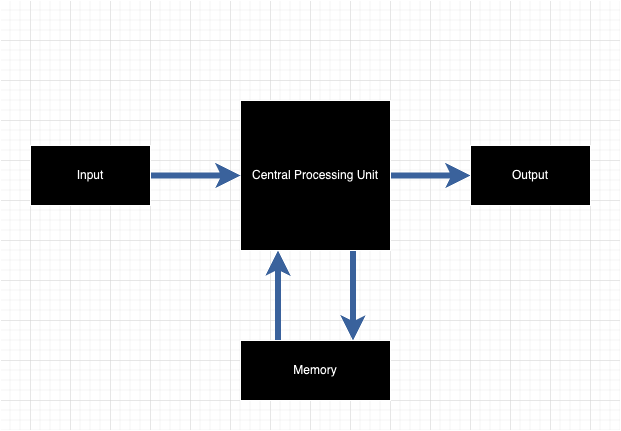
\includegraphics[width=\textwidth]{neumann}
\caption{Von Neumann Architecture}
\end{figure}
\\
That is, they take input, process it and produce output. Input can come either directly from the user through peripheral devices, or from data stored in the system's main memory. The system can also store and retrieve data in memory. In order to speed up memory access, systems have a memory hierarchy called a cache. Data immediately being used by the system is stored in CPU registers. Beyond this, the CPU has L1, L2 and sometimes L3 cache, and further beyond this the system has its main memory (RAM), and even the hard drive. The memory stores of this hierarchy become progressively large, but also progressively slower to access.\\
\begin{figure}[h]
	\centering
	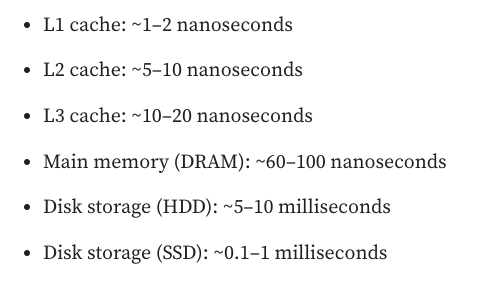
\includegraphics[width=8cm]{access_time}
	\caption{Approximate time to access various memory types \cite{accessTime}}
\end{figure}
\pagebreak
\\
When a program is compiled and run it is allotted a certain amount of memory automatically, this is called its stack. A common use case for the stack is function calls. When a program calls a function, local variables inside the new function need to be stored somewhere. The program also needs to know, when the function ends, which location to return back to \cite{10.5555/202036}.\\
\\
\begin{figure}[h]
	\centering
	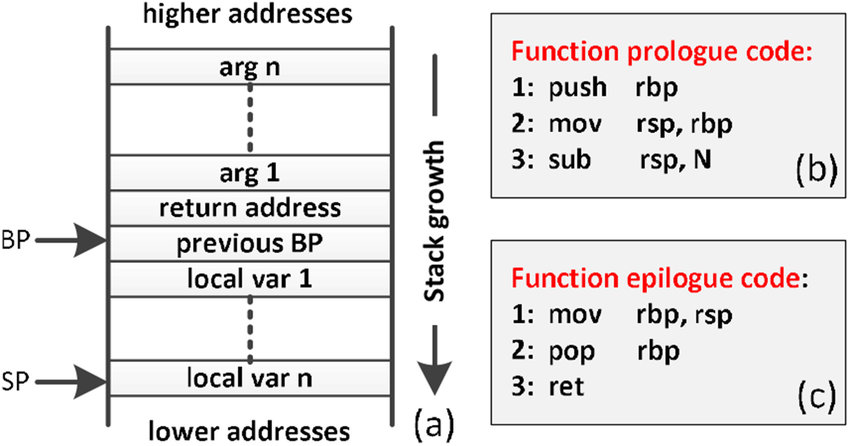
\includegraphics[width=8cm]{stack_frame}
	\captionsetup{width=10cm}
	\caption{Example stack usage for function call. Arguments are stored in reverse order so arbitrary numbers of arguments can be handled. The function prologue and epilogue are called at the beginning and end of the function respectively in order to save and restore the return address. \cite{stackFrame}}
\end{figure}
\\
In addition to use cases like this,  it's possible (and quite fast) to allocate memory from the stack. However, since the stack is allocated to  the program at compile time, it is not intended to handle large runtime allocations and is limited to the order of a few megabytes. Excessive stack allocations can cause stack overflows and crash a program.\\
\\
For general runtime allocations, the application programmer also has access to the system heap. In contrast to the heap data structure, the system's memory heap is the phrase used to describe all the memory which a system has access to \cite{knuth97}. The heap is the most common source from which memory is allocated at runtime. Heap allocation is more flexible, but involves a call to the operating system and higher overheads, as the heap is shared by many other programs running simultaneously on the system, possibly simultaneously using the same physical memory (thanks to virtual memory).\\
\\
A memory allocation can be visualized as a pointer to the beginning of a region of memory, with the guarantee that only this pointer will have exclusive ownership over that region. Many allocators have the same public interface as C's standard library, namely the functions \\
\begin{lstlisting}[language=C]
void* malloc(size_t byteSize);
\end{lstlisting}
and 
\begin{lstlisting}[language=C]
void free(void* location);
\end{lstlisting}
which allocate and free memory respectively. Internally, many allocators also share similar mechanisms. An allocator will typically request some region of memory from the operating system at the beginning of the program, and then use some sort of data structure to partition that region to satisfy runtime allocations. It is common to name these sub regions "blocks".\\
\\
Upon a memory request, the allocator will attempt to find a free block which is able to satisfy the request. Some allocators deal with fixed sizes and others are flexible. It's common to split blocks so that the unused space can be used for future allocations.
\\
\begin{figure}[h]
	\centering
	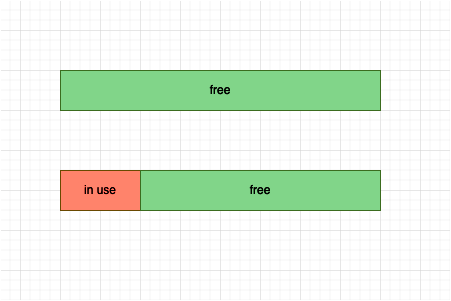
\includegraphics[width=10cm]{split}
	\captionsetup{width=10cm}
	\caption{Splitting a block}
\end{figure}
\\
Over the runtime of the program, memory which was previously allocated may be freed. In these cases, a custom allocator should have some mechanism to detect when neighbouring blocks can be merged together into one, larger free block. This merging process is called ``coalescing''.\\
\\
\begin{figure}[h]
	\centering
	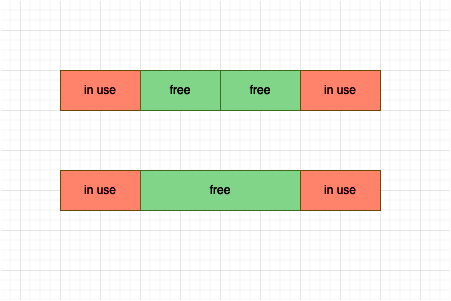
\includegraphics[width=10cm]{coalesce}
	\captionsetup{width=10cm}
	\caption{Memory Coalescing}
\end{figure}
\\
The fundamental problem with dynamic memory allocation is it is dynamic. Over the lifetime of the program, an allocator's initial slab of memory may undergo many modifications. These modifications can make regions of memory unusable, this is known as fragmentation. Fragmentation comes in two forms, external fragmentation occurs when free blocks exist which cannot be coalesced together. Although the allocator has enough free memory, it may still fail to satisfy requests due to not having a large enough free block.\\
\\
\begin{figure}[h]
	\centering
	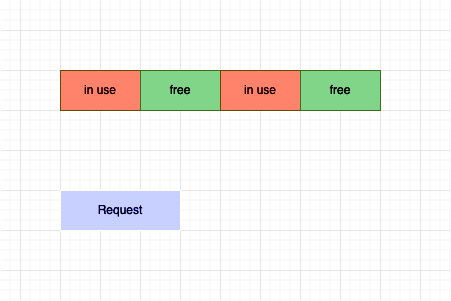
\includegraphics[width=10cm]{external_fragmentation}
	\captionsetup{width=10cm}
	\caption{External fragmentation}
\end{figure}
\\
Internal fragmentation describes the scenario where the allocator marks off a larger block than requested, does not split, and hence leaves some portion of a block unused. This may come about due to memory alignment/padding requirements, or the allocator's own mechanism. For instance fixed-size allocators exist which will not split blocks.\\
\\
\begin{figure}[h]
	\centering
	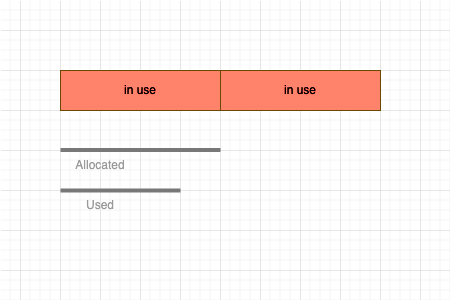
\includegraphics[width=10cm]{internal_fragmentation}
	\captionsetup{width=10cm}
	\caption{Internal fragmentation}
\end{figure}
\\
Cache friendly programming can make a big difference to performance. As noted previously, in practice the Central Processing Unit attempts to fulfill fetches with its cache. Memory is not fetched a byte at a time, but by cache lines, typically 64 bytes. This means that if an application programmer is able to maximise the amount of ``useful data'' per cache line, the program will probably run faster. For instance, a linked list typically involves a number of nodes, each with a pointer to other nodes. If an allocator allocates space for these nodes at random locations on the heap then a lot of time is wasted traversing the list as each pointer access means fetching a new cache line. Furthermore, if the allocator allocates nodes fairly close together in memory, but incurs internal fragmentation, then the amount of useful data per cache line is reduced, and traversal may involve more cache ejections and refreshes than necessary. Though such allocators may satisfy requests quickly, the memory they allocate can still be slow to access.\\
\\
Some memory requests can also request the returned pointer be a multiple of a number, usually a power of two. This practice is called memory alignment. Although modern CPUs can mitigate this problem, misalignment can lead to less efficient memory access, as the memory may be needlessly split across two cache lines. The idea of memory alignment is to introduce some necessary padding so that the address becomes a multiple of the requested alignment \cite{allignment}:\\
\\
$padding = \left(align - \left(address\ mod\ align\right)\right)\ mod\ align$\\
$aligned = address + padding$\\
\pagebreak
Since the alignment is a power of two, the modulus operator can reduce to a bitwise and which clears off all bits above and including the align bit.\\
$padding = \left(align - \left(address\ \&\ \left(align - 1\right)\right)\right)\ \&\left(align - 1\right)$\\
$\hspace*{1cm} = \left(\left(align\ \& \left(align - 1\right)\right) - \left(address\ \&\ \left(align - 1\right)\right)\right)\ \&\left(align - 1\right)$\\
$\hspace*{1cm} = \left(0 - \left(address\ \&\ \left(align - 1\right)\right)\right)\ \&\left(align - 1\right)$\\
$\hspace*{1cm} = \left(\neg\left(address\ \&\ \left(align - 1\right)\right) + 1\right)\ \&\left(align - 1\right)$\\
$\hspace*{1cm} = \left(\left(\neg address\ \lor\ \neg\left(align - 1\right)\right) + 1\right)\ \&\left(align - 1\right)$\\
$\hspace*{1cm} = \left(-address\ \lor\ \neg\left(align - 1\right)\right)\ \&\left(align - 1\right)$\\
$\hspace*{1cm} = \left(-address\ \&\left(align - 1\right)\right)\ \lor\ \left(\neg\left(align - 1\right)\ \&\left(align - 1\right)\right)$\\
$\hspace*{1cm} = \left(-address\ \&\left(align - 1\right)\right)\ \lor\ 0$\\
$\hspace*{1cm} = -address\ \&\left(align - 1\right)$\\
This padding can then be added to the requested address to ensure it is correctly aligned.

\section{Previous Work}
Knuth's work \cite{knuth97} is considered the classic introduction to memory allocation algorithms. Here, the fundamental data structures, namely free list and buddy allocators, are discussed.\\
\\
\begin{figure}[h]
	\centering
	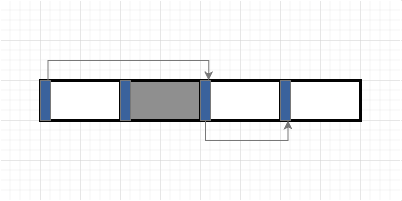
\includegraphics[width=10cm]{list_allocator}
	\captionsetup{width=10cm}
	\caption{A linked-list representation of memory. Each header links to the header for the next free block. Neighbouring blocks can be found using block sizes.}
\end{figure}
\\
Free list allocators are based around the idea of linked lists, each node in the linked list describes a region of memory, for instance its size, padding and whether it is currently free or in use. Two free list algorithms are presented by Knuth: first fit and best fit. First fit traverses a linked list of free nodes to find the first one which is large enough to satisfy the request. Best fit searches the whole list to find the smallest such node. Both of these strategies are linear in their worst case execution time, which may not be desired for large systems.\\
\pagebreak
\begin{figure}[h]
	\centering
	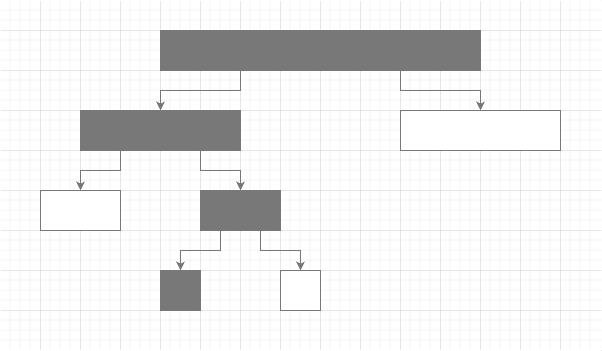
\includegraphics[width=10cm]{buddy_allocator}
	\captionsetup{width=10cm}
	\caption{A buddy allocation system, represented here with a binary tree.}
\end{figure}
\\
Knuth also discusses buddy systems, these are similar except that blocks are split in half until a suitable size is allocated. Buddy systems can be made faster than free lists by imposing a binary search tree structure, giving them logarithmic search time. Knuth also mentions the benefit of immediately freeing memory over garbage collection.\\
\\
In the following years some incremental progress has been made on these fundamental algorithms. Hosking, Moss and Jones \cite{10.5555/2025255} summarise some of these in the Garbage Collection Handbook. The concepts of size classes are discussed, along with the internal fragmentation problem of buddy allocators. Some more advanced data structures such as splay trees, Cartesian trees and bitmap fits are presented. The authors also briefly discuss considerations for multi threaded allocation, however such a topic is out of scope for this project. At any rate the authors conclude that most of the gains of multi threading can be realised by having well designed single thread allocators run independently.\\
\begin{figure}[h]
	\centering
	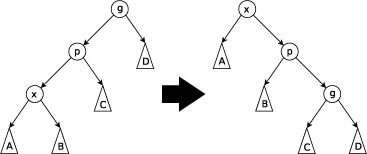
\includegraphics[width=9cm]{splay_tree}
	\captionsetup{width=10cm}
	\caption{A splay tree, before and after searching for node x.}
\end{figure}
\\
Splay Trees, first proposed by Sleator and Tarjan \cite{10.1145/3828.3835}, are binary search trees where upon search, the result is promoted to the root of the tree. This has the benefit that frequently searched nodes are ``hot'' in memory and require less work to retrieve in future searches. 
\pagebreak
\begin{figure}[h]
	\centering
	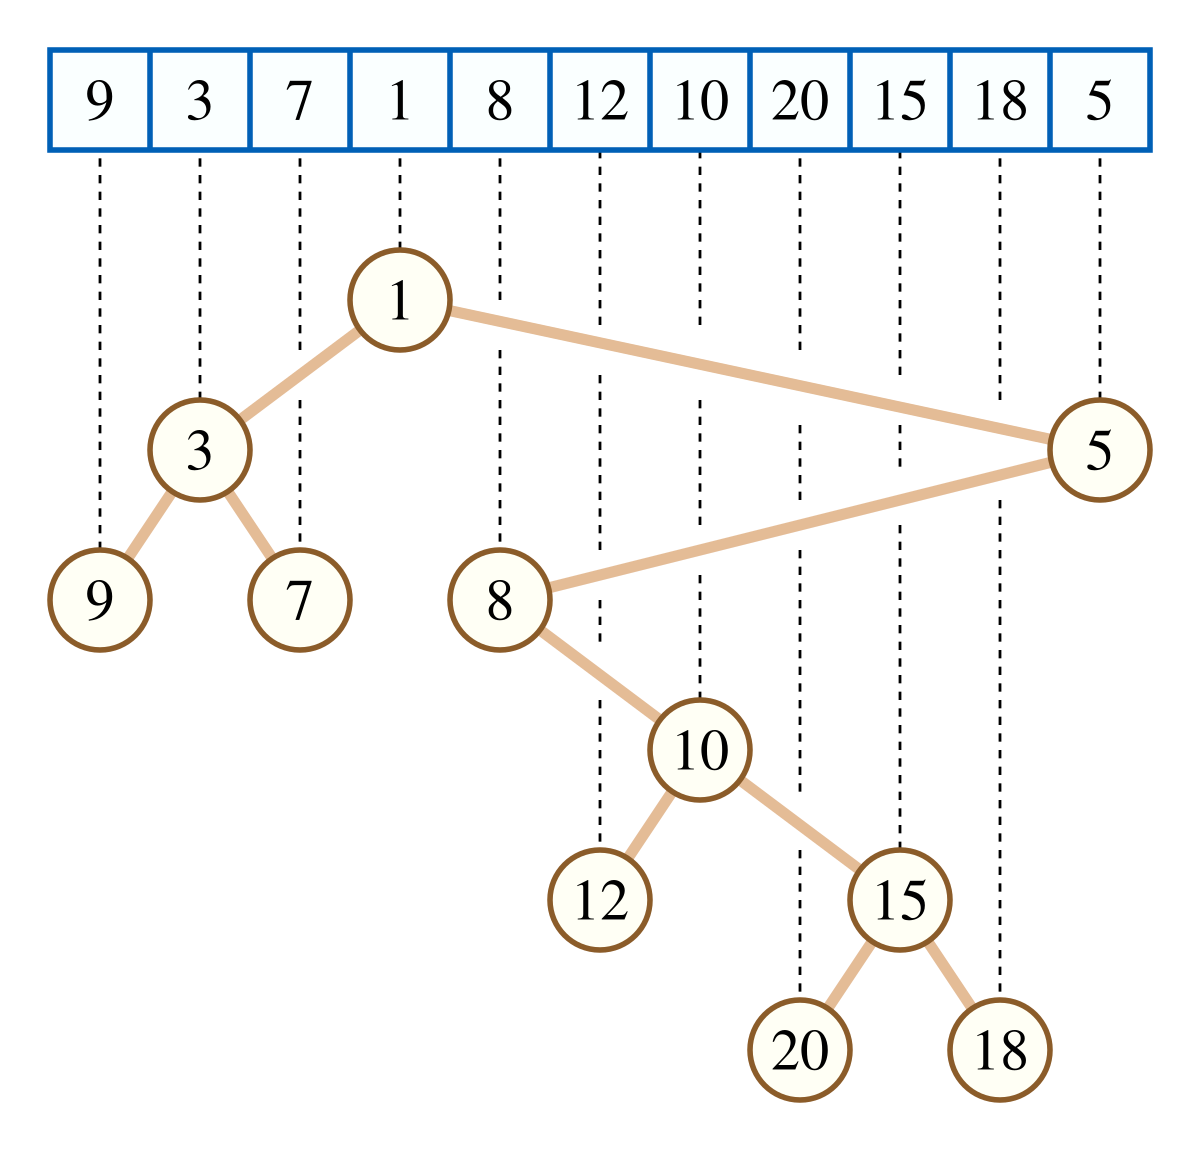
\includegraphics[width=9cm]{Cartesian_tree}
	\captionsetup{width=10cm}
	\caption{A Cartesian tree, x axis represents memory location, y axis represents value.}
\end{figure}
\\
Cartesian trees, presented by Vuillemin \cite{10.1145/358841.358852}, are a two dimensional generalization of search trees. In a Cartesian tree, addresses are ordered from left to right and sizes are ordered from top to bottom. This has the advantage that the root node has the highest block size, and requests which are too large can be quickly rejected. A notable constraint of Cartesian trees is the inability to be re-balanced, and so the probablilty of highly unbalanced trees with linear search time can increase. This makes the worst case execution time difficult to predict.\\
Stephenson proposes a memory allocator based on Cartesian Trees in \cite{10.1145/800217.806613}, named ``Fast Fits''. Stephenson found that Fast Fits performs somewhere between Free Lists with Buddy Allocators. Although neither Cartesian nor Splay trees were investigated in this report, they are novel approaches which could be examined in future work.\\
\\
\begin{figure}[h]
	\centering
	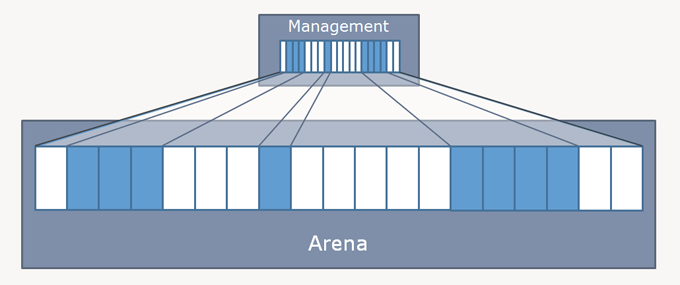
\includegraphics[width=9cm]{arena_allocator}
	\captionsetup{width=10cm}
	\caption{Separating headers from blocks}
\end{figure}
\\
As mentioned previously, maximising the amount of useful data per cache line will tend to make programs run faster, the same principle holds for the data structure used to track blocks. As such, a number of allocators have been developed which separate the block headers from the blocks they manage.\\
\\
Matani and Menghali \cite{matani2021fastbitmapfitcpu} propose such an allocator which takes this concept even further. A fast bitmap fit allocator encodes a small binary search tree directly into the bits of an integer. The proposed allocator can quickly search, allocate and free as the whole structure is cache-local. The allocator can also take a "hint" to attempt adjacent allocations. In this system, all searches, allocations and frees can be done with bit level operations on a single unsigned integer, making the search structure very fast. As a trade-off, the allocator is more limited. A certain maximum number of allocations can be made (at least in the naive form), and allocations must all be fixed size. This approach is interesting for fixed size object pools, but may be limited in its use cases.\\
\\
\begin{figure}[h]
	\centering
	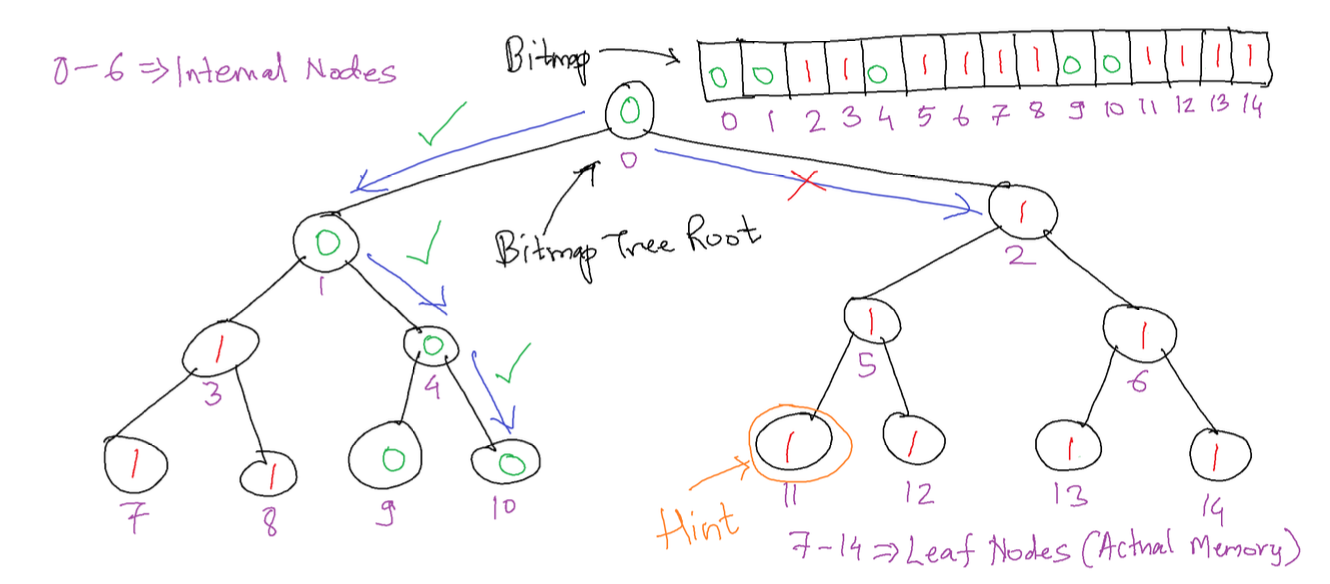
\includegraphics[width=10cm]{bitmap_allocator}
	\captionsetup{width=10cm}
	\caption{Bitmap allocator, leaf nodes represent actual memory blocks. Algorithm chooses search directions at each level in order to minimise the distance to the allocation hint.}
\end{figure}
\\
A big limitation with the allocators discussed so far is not necessarily their execution time, but the predictability of their worst case execution times. Real time systems need some guarantee that a task will complete within a bounded interval of time, and so a number of allocators have been proposed which guarantee this.\\
Ogasawara proposed a constant time allocator in \cite{528746} which maintains an array of free lists, each corresponding to a size class in the range $\left[2^i, 2^{i + 1}\right)$. This keeps size classes flexible and enforces the condition that every block on the list must be able to fulfill a request. This means that memory requests do not require searching a free list or binary tree, provided the free list has a block, that block will be appropriate. Upon allocation, blocks can be split, reducing internal fragmentation. While internal fragmentation is reduced, this can still have the effect of scattering memory allocations randomly through memory.\\
\\
Ogasawara's constant time allocator is based on ``power of two'' size classes, this covers a wide range of sizes but is fairly coarse. Linear size classes can fill in gaps but are difficult to effectively search for large ranges of sizes. Knuth had experimented with multi-level allocators but did not achieve satisfactory results, nonetheless commenting that multi level allocators were theoretically possible.\\
Masmano, Ripoli, Crespo and Real \cite{inproceedings} developed a two level structure which they called the Two Level Segregated Fit (TLSF). This allocator manages a first level which holds ``power of two'' size classes. Each first level size class links to a second level, an array of linear size classes. The power of this structure is not in its concept, but its execution. Every memory size can be mapped to an underlying free list via the coordinates $\left(f,s\right)$:\\
$f := \lfloor\log_2\left(size\right)\rfloor$\\
$s := \left(size - 2^f\right) \frac{2^{SLI}}{2^f}$\\
Where $SLI$, the second level index, is a parameter which describes how many second levels each first level size class is split into. It turns out that $\left(f, s\right)$ can be computed with bit-level operations. The authors describe some further optimisations, chief among them: by restricting the number of first and second level size classes to 32 at most, integers can be used to track the free status of each size class, reducing the work to search for available free lists able to satisfy $\left(f, s\right)$. Using integers also restricts the worst case search time.\\
TLSF is considered a good general allocator, especially in real time systems. Elegant in its design and fairly flexible, perhaps its only shortcoming is a lack of multi threading  support, which is out of scope for this project.\\
\\
While the development of allocation algorithms is important, the ability to benchmark allocators is equally so. Traditionally this was done with asymptotic analysis. While a good tool, this is not the only important metric. With the development of instruction-level profiling tools, it became possible to measure exactly how much work an allocator was doing. Detlefs, Dosser and Zorn \cite{10.1002/spe.4380240602} published one such paper where various memory allocators were compared for a variety of real malloc-heavy applications, by counting the number of instructions used for allocation and free operations.\\
One of the chief conclusions of the paper was that a well designed garbage collected allocator could compete with manual memory managers. Although the authors acknowledged that the programs themselves took significantly longer to run with garbage collection, possibly due to a trade off between Garbage Collection overhead (running more frequently) and external fragmentation (running less frequently). Nevertheless, the concept of measuring clock cycles for allocators was an important step forwards.\\
\\
Fragmentation (both internal and external) can have an effect on system performance. Both by wasting space and by scattering useful data. Therefore it is important to have some means of estimating an allocator's fragmentation rate. Previously, fragmentation was measured by synthetic trace analysis. That is, randomly generating a series of malloc and free calls, then replaying that. In some cases great efforts were taken to ensure traces had statistically significant properties. Johnstone and Wilson \cite{10.1145/301589.286864} re-examined the implicit assumption in these benchmarks: that synthetic trace analysis is an indicator of fragmentation in real programs, and found this not to be true.\\
\\
The authors used a journal replay method. Real programs were executed which logged requests to file, this gave a real trace to be analysed. This ``Memory Journal'' could then be replayed, and at any point an allocator's total unusable memory and requested memory could be queried and compared as a means of estimating fragmentation. It was found that in real use cases, fragmentation rates were lower than previously predicted, and acceptable for most allocators. In addition to challenging synthetic trace analysis, another goal of the study was to evaluate allocator policies independent of implementation. The authors concluded that immediate coalescing on free and reuse of most frequently freed blocks gives best performance.\\
\\
Previous research by Grunwald and Zorn had profiled allocators on the basis of instruction counts, but this neglects the possibility that an allocator's allocation or free time may be independent of how fast the allocated memory is to use. Grunwald, Zorn and Henderson wrote a follow up paper \cite{10.1145/173262.155107} with the aim of investigating the relationship between allocator and execution time for a number of real programs. More specifically, they attempted to measure cache occupancy. This sort of research into cache hit rates had only previously been undertaken for Garbage Collected languages, where its effect was obvious. It was concluded that the choice of allocator effects both cache hit rate and total execution time for a number of allocation-heavy programs, but that there isn't a single implementation which is universally best for every program.

\section{In Practice}
In order to see how some of this theory might work in practice I decided to recreate a blog post by Forrest Smith \cite{doom3-malloc}. Smith wanted to challenge the notion that the standard C malloc routine is slow by profiling it on a real, open source program, Doom 3. The experimental design went as follows:\\
\begin{itemize}
	\item Modify the allocate and free functions in Doom 3 source code to write a description of the request to a memory journal.
	\item For a number of different allocators, replay the journal, timing each allocation or free operation
	\item Plot the results, do some statistical analysis
\end{itemize}

I downloaded the same source port as Smith and got it running with the proper assets. I also identified the point at which to log info out, though unfortunately some further modification would be needed to enable the program to write out to files. Determining that my goal was to profile allocators rather than produce an original trace, I downloaded Smith's memory journal and used that. Journal lines had the format: \\
\begin{lstlisting}
	//a size pointer threadID timestamp
	a 2048 000002C453C48560 7360 329200
\end{lstlisting}
for allocations, or\\
\begin{lstlisting}
	//f pointer threadID timestamp
	f 000002C453C17290 7360 911600
\end{lstlisting}
for frees.
\\
I designed an abstract allocator class with the following interface:\\
\begin{lstlisting}[language=C++]
class Allocator{
	public:
	virtual void* custom_malloc(size_t size, size_t alignment) = 0;
	virtual void* custom_realloc(size_t size, 
					size_t alignment,  
					void* oldAddress) = 0;
	virtual void custom_free(void* data, bool debug) = 0;
	std::string name;
};
\end{lstlisting}
This could then be used for journal replay (full listing in Appendix A)
\begin{lstlisting}[language=C++]
void benchmark(Allocator& allocator) {
	
	// Local variables to track active allocations, allocation sizes etc.
	// ...
	
	// pre read and count the number of allocations and frees
	std::ifstream journal;
	journal.open("../data/doom3_journal.txt");
	int64_t malloc_count = 0, free_count = 0;
	while (std::getline(journal, line)) {
		
		// ...
		
	}
	
	// data sets for results.
	// x axis: timestamp
	// y axis: duration
	// color: size
	// ...
	
	while (std::getline(journal, line)) {
		std::vector<std::string> words = split(line, " ");
		
		if (words[0].compare("a") == 0) {
			//allocate
			//...
			
			//---- time this ----//
			auto start = std::chrono::high_resolution_clock::now();
			void* data = allocator.custom_malloc(size, 16);
			auto end = std::chrono::high_resolution_clock::now();
			float duration = std::chrono::
			duration_cast<std::chrono::nanoseconds>(end - start).count();
			//-------------------//
			
			//---- log ----//
			// ...
			//------------//
			
		}
		
		if (words[0].compare("f") == 0) {
			//free
			//...
			
			//---- time this ----//
			auto start = std::chrono::high_resolution_clock::now();
			if (data) {
				allocator.custom_free(data);
			}
			auto end = std::chrono::high_resolution_clock::now();
			float duration = std::chrono::
			duration_cast<std::chrono::nanoseconds>(end - start).count();
			//-------------------//
			
			//---- log ----//
			//...
			//------------//
		}
	}
	
	// Write back results
	std::ofstream file;
	std::stringstream filename_builder;
	
	filename_builder << "../data/" << allocator.name << "_allocate.txt";
	file.open(filename_builder.str(), std::ofstream::out);
	for (size_t j = 0; j < malloc_count; ++j) {
		file << ...;
	}
	file.close();
	
	filename_builder.str("");
	filename_builder << "../data/" << allocator.name << "_free.txt";
	file.open(filename_builder.str(), std::ofstream::out);
	for (size_t j = 0; j < free_count; ++j) {
		file << ...;
	}
	file.close();
}

int main() {
	FreeListAllocator bestFitList(FreeListAllocator::PlacementPolicy::FIND_BEST);
	benchmark(bestFitList);
	return 0;
}
\end{lstlisting}
I implemented an allocator based on C's standard library (See Appendix B), and found two more online, a TLSF \cite{TLSF-implementation} and linear free list allocator \cite{free-list-implementation}. Some adaptation was necessary in order for them to comply with the abstract allocator.\\
\\
I then plotted the results in python.\\
\begin{lstlisting}[language=Python]
import numpy as np
import matplotlib.pyplot as plt
	
data = np.loadtxt("data/TLSF_allocate.txt", delimiter=" ")
	
timestamp = vanilla_alloc_data[:,0]
time = vanilla_alloc_data[:,1]
size = vanilla_alloc_data[:,2]

valid_indices = time != 0
	
x = timestamp[valid_indices]
y = np.log10(time[valid_indices])
c = np.log2(size[valid_indices])
	
y_ticks = [1, 2, 3, 4, 5, 6]
y_labels = ["10ns", "100ns", "1us", "10us", "100us", "1ms"]
	
c_ticks = [1, 2, 3, 4, 5, 6, 7, 8, 9, 10,
	11, 12, 13, 14, 15, 16, 17, 18, 19, 20,
	21, 22, 23, 24, 25, 26, 27, 28, 29, 30,]
c_labels = ["", "4 b", "", "16 b", "", "64 b", "", "256 b", "", "1 kb",
	"", "4 kb", "", "16 kb", "", "64 kb", "", "256 kb", "", "1 mb",
	"", "4 mb", "", "16 mb", "", "64 mb", "", "256 mb", "", "1 gb",]
	
thing = plt.scatter(x = x, y = y, c = c, s = 0.2, cmap="gist_ncar")
plt.yticks(ticks=y_ticks, labels=y_labels)
cbar = plt.colorbar(ticks=c_ticks)
cbar.set_ticklabels(c_labels)
plt.tight_layout()
plt.show()
\end{lstlisting}
\pagebreak
To produce the following graphs:\\
\begin{figure}[h]
	\centering
	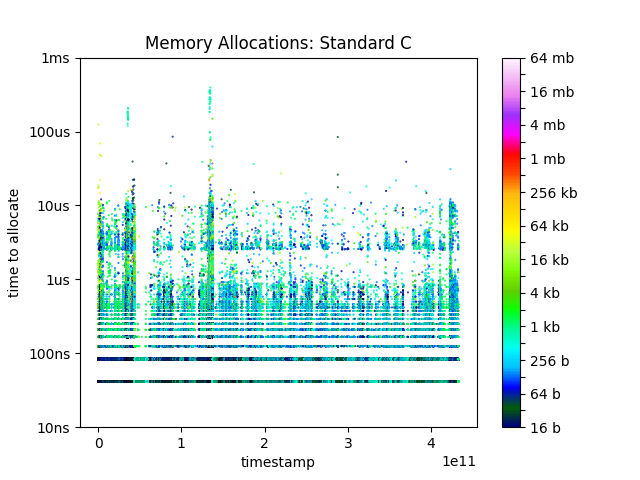
\includegraphics[width=10cm]{results_vanilla_alloc}
	\captionsetup{width=10cm}
	\caption{Standard C allocator}
\end{figure}
\begin{figure}[h]
	\centering
	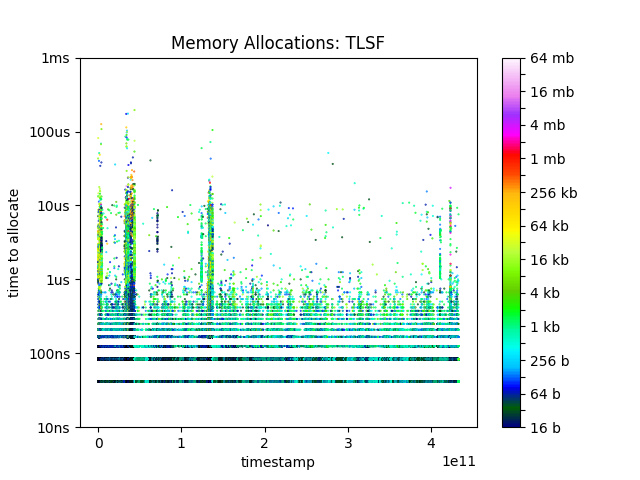
\includegraphics[width=10cm]{results_tlsf_alloc}
	\captionsetup{width=10cm}
	\caption{Two Level Segregated Fit allocator}
\end{figure}
\begin{figure}[h]
	\centering
	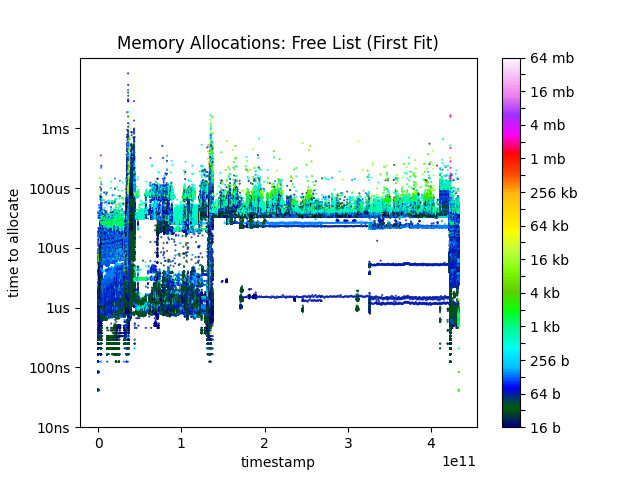
\includegraphics[width=10cm]{results_first_alloc}
	\captionsetup{width=10cm}
	\caption{Free List allocator (first fit strategy)}
\end{figure}
\begin{figure}[h]
	\centering
	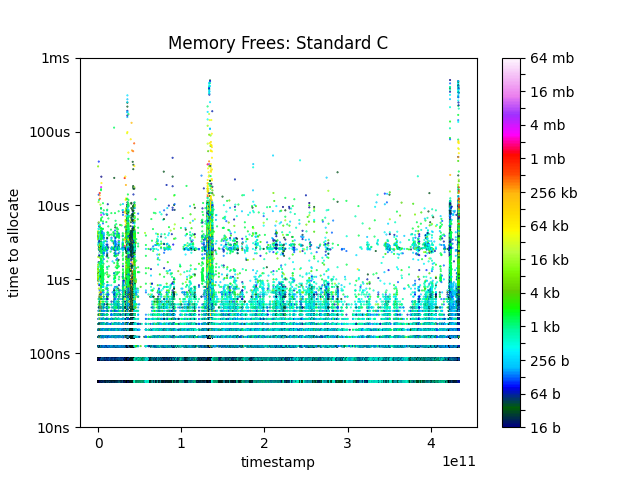
\includegraphics[width=10cm]{results_vanilla_free}
	\captionsetup{width=10cm}
	\caption{Standard C allocator}
\end{figure}
\begin{figure}[h]
	\centering
	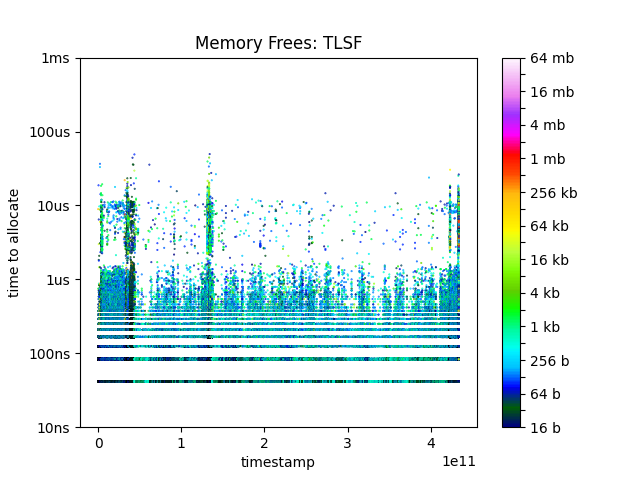
\includegraphics[width=10cm]{results_tlsf_free}
	\captionsetup{width=10cm}
	\caption{Two Level Segregated Fit allocator}
\end{figure}
\begin{figure}[h]
	\centering
	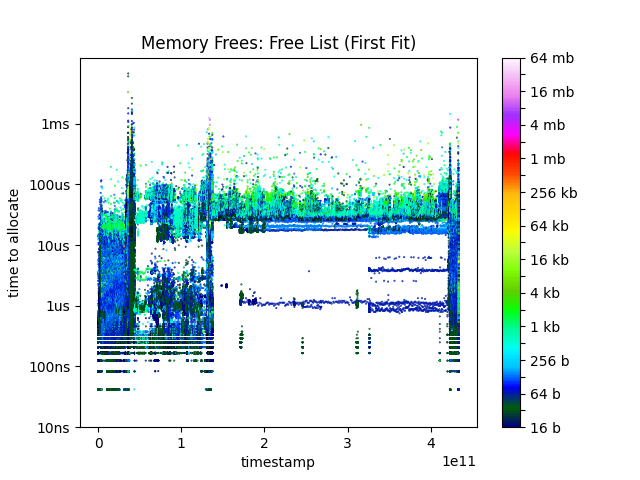
\includegraphics[width=10cm]{results_first_free}
	\captionsetup{width=10cm}
	\caption{Free List allocator (first fit strategy)}
\end{figure}
\\
From these it seems that allocation and freeing have similar behaviour, Free Lists take an exceptional amount of time, and TLSF performs similarly to C's standard library, but with less variance. This can be further investigated with box and whisker plots.\\
\\
\begin{figure}[h]
	\centering
	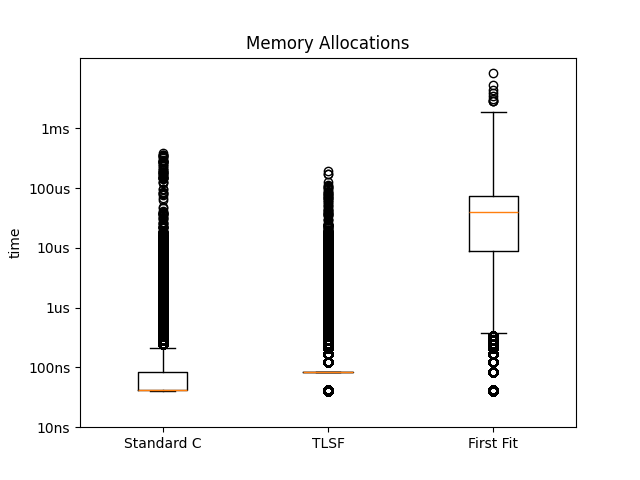
\includegraphics[width=10cm]{boxplots_allocate}
	\captionsetup{width=10cm}
	\caption{Memory Allocation times}
\end{figure}
\begin{figure}[h]
	\centering
	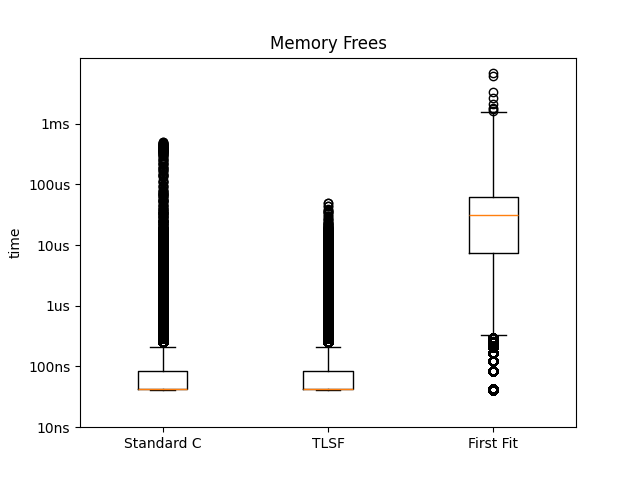
\includegraphics[width=10cm]{boxplots_free}
	\captionsetup{width=10cm}
	\caption{Memory Free times}
\end{figure}
\\
From these distributions we can see that TLSF is incredibly consistent for allocations, and otherwise more or less matches C's standard library allocator. As seen in the initial graphs, First fit is an extremely slow allocator for a real time system.

\section{Strategies}
We could look at the results above and conclude something along the lines of: the standard library does a pretty good job. We could use a TLSF allocator if performance is critical and we have time to spend on debugging and tuning. Such a conclusion would be perfectly reasonable, but it skips a big question: do we need a dynamic memory allocator?\\
\\
As mentioned previously, the problem with dynamic memory allocation is that it is dynamic. Hence, the solution to dynamic memory allocation could be not to allocate memory dynamically. Consider the distribution of sizes for all the allocation requests in the Doom 3 memory journal.\\
\\
\begin{figure}[h]
	\centering
	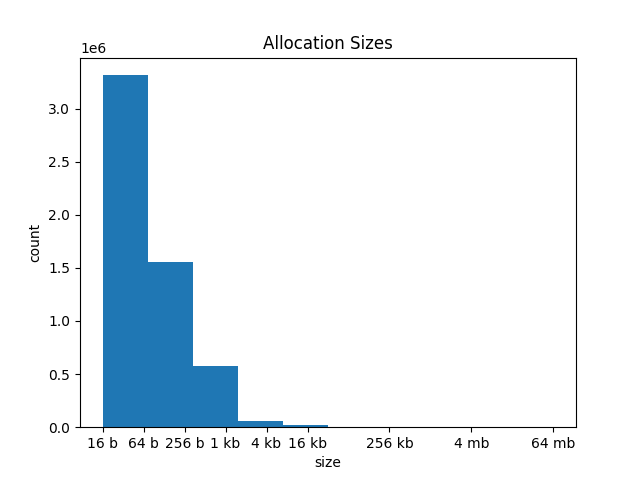
\includegraphics[width=10cm]{size_distribution}
	\captionsetup{width=10cm}
	\caption{Distribution of requested sizes}
\end{figure}
\\
During its short runtime, the program has made a very large number of small allocations, most commonly 16 bytes. While a dynamic allocator can make this approach possible, it runs the very real risk of scattering data randomly in memory and needlessly driving up overheads on allocation calls. Before a fully dynamic allocation is made, there are a number of strategies which can be considered.\\
For short lived memory, in the order of a few kilobytes or less, stack allocation is viable. C's alloca and free can achieve this. Allocating on the stack ensures that the memory locations are fairly close together. Also since it involves incrementing the stack pointer rather than searching a data structure, it is fairly fast.\\
\\
For objects such as linked lists, it can be viable to allocate some amount of backing memory to hold the nodes, reallocating if needed. Not only does this reduce the number of allocation calls, but it also ensures fast traversal. For small collections of objects, a pool or fixed size allocator may be beneficial.\\
\\
Rather than individual objects, abstract collection objects can be used to group resources. These go by a few names such as ``Managed Arrays'', ``Vectors'', ``Component Sets'' or ``Arena Allocators''. In all cases the idea is the same, some object creates and manages backing memory. Upon resize, doubling the size of the backing memory further reduces the number of reallocations, at the expense of allocating more memory than needed.\\
\\
Rethinking the way the program decomposes into subsystems, each subsystem can manage its backing memory. This also has the benefit of making a program's memory footprint more predictable.\\

\section{Conclusion}
In this project I have presented the problem of dynamic memory allocation, along with the related concepts and terminology. I've discussed some of the work which has been undertaken in the field, and benchmarked some allocators in a practical scenario.  I've also presented a number of recommendations for strategies to try before reaching for a dynamic memory allocator. As many other studies have likewise concluded, there is no universal solution to all memory allocation problems. In fact, many more benefits can be realised by designing systems so as to rely less on dynamic allocation.
As a final, motivating example, here is a simple Python Raytracer I made in order to stress test my CPU.\\
\\
\begin{figure}[h]
	\centering
	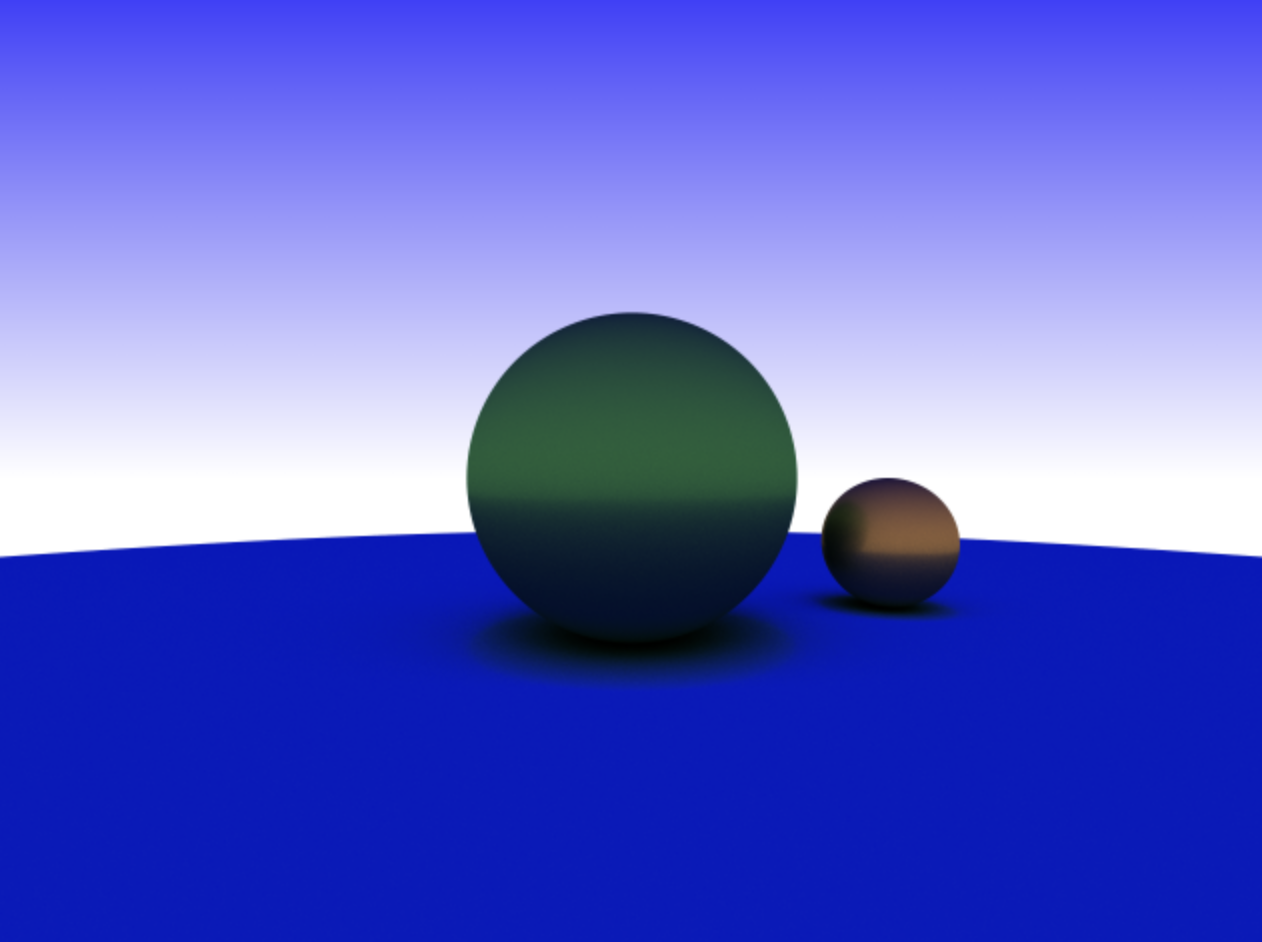
\includegraphics[width=10cm]{raytrace}
	\captionsetup{width=10cm}
	\caption{A CPU raytracer.}
\end{figure}
\\
Rendering one scene, with 2048 samples per ray, and every ray rebounding up to 2048 times takes 55 minutes on a Mac M1 Pro. Python does not have a concept of stack allocation, so each local variable is a small heap allocation, incurring all the associated pitfalls. Replacing local variables with a single list of floating point numbers, which is created once at the start of the program and then passed around in arguments as a sort of ``scratchpad'' reduces execution time to 45 minutes. It is not monumental, but it is enough to prove that memory matters.

\bibliography{bibbed}{}
\bibliographystyle{plain}

\begin{appendices}
	\section[A]{Source Code for Journal Replay}
	\begin{lstlisting}[language=C++]
#include "allocators/allocator.h"
#include "allocators/vanilla/vanilla.h"
#include "allocators/free_list/free_list.h"
#include "allocators/tlsf/tlsf.h"
#include <fstream>
#include <vector>
#include <unordered_map>
#include <cstdint>
#include <sstream>
#include <iostream>
#include <chrono>
	
std::vector<std::string> split(std::string line, std::string delimiter) {
	
	std::vector<std::string> words;
		
	size_t pos = 0;
	std::string token;
	while((pos = line.find(delimiter)) != std::string::npos) {
		token = line.substr(0,pos);
		words.push_back(token);
		line.erase(0, pos + delimiter.length());
	}
	words.push_back(line);
		
	return words;
}
	
void benchmark(Allocator& allocator) {
		
	std::cout << "---- Benchmark " << allocator.name << " Allocator ----" << std::endl;
	std::string line;
	std::unordered_map<std::string, void*> allocations;
	std::unordered_map<std::string, size_t> sizes;
	size_t size;
	std::string ptr;
	std::string threadID;
	std::string timestamp;
	float malloc_average = 0;
	float free_average = 0;
		
	// pre read in order to allocate
	std::ifstream journal;
	journal.open("../data/doom3_journal.txt");
	int64_t malloc_count = 0, free_count = 0;
	while (std::getline(journal, line)) {
			
		std::vector<std::string> words = split(line, " ");
			
		if (words[0].compare("a") == 0) {
			malloc_count++;
		}
		if (words[0].compare("f") == 0) {
			free_count++;
		}
			
	}
	journal.close();
	journal.open("../data/doom3_journal.txt");
		
	float malloc_coefficient = 1.0f / malloc_count;
	float free_coefficient = 1.0f / free_count;
		
	// x axis: timestamp
	// y axis: duration
	// color: size
	std::vector<float> x_a(malloc_count);
	std::vector<float> y_a(malloc_count);
	std::vector<float> c_a(malloc_count);
	std::vector<float> x_f(free_count);
	std::vector<float> y_f(free_count);
	std::vector<float> c_f(free_count);
		
	while (std::getline(journal, line)) {
		std::vector<std::string> words = split(line, " ");
			
		if (words[0].compare("a") == 0) {
			//allocate
			//a size ptr threadID timestamp
			std::stringstream converter(words[1]);
			converter >> size;
			ptr = words[2];
			threadID = words[3];
			timestamp = words[4];
				
			//---- time this ----//
			auto start = std::chrono::high_resolution_clock::now();
			void* data = allocator.custom_malloc(size, 16);
			auto end = std::chrono::high_resolution_clock::now();
			float duration = std::chrono::
			duration_cast<std::chrono::nanoseconds>(end - start).count();
			malloc_average += malloc_coefficient * duration;
			//-------------------//
				
			//---- log ----//
			x_a[i] = std::stof(timestamp);
			y_a[i] = duration;
			c_a[i++] = static_cast<float>(size);
			//------------//
				
			allocations[ptr] = data;
			sizes[ptr] = size;
				
		}
		
		if (words[0].compare("f") == 0) {
			//free
			//f ptr threadID timestamp
			ptr = words[1];
			threadID = words[2];
			timestamp = words[3];

			void* data = allocations[ptr];
			//std::cout << data << std::endl;
			allocations.erase(ptr);
			//---- time this ----//
			auto start = std::chrono::high_resolution_clock::now();
			if (data) {
				allocator.custom_free(data);
			}
			auto end = std::chrono::high_resolution_clock::now();
			float duration = std::chrono::
			duration_cast<std::chrono::nanoseconds>(end - start).count();
			free_average += free_coefficient * duration;
			//-------------------//
				
			//---- log ----//
			x_f[i2] = std::stof(timestamp);
			y_f[i2] = duration;
			c_f[i2++] = static_cast<float>(sizes[ptr]);
			//------------//
		}
	}
		
	std::cout << "Allocation time (average): " 
		<< malloc_average << " ns." << std::endl;
	std::cout << "Free time (average): " 
		<< free_average << " ns." << std::endl;
		
	// Write back results
	std::ofstream file;
	std::stringstream filename_builder;
	
	filename_builder << "../data/" << allocator.name << "_allocate.txt";
	file.open(filename_builder.str(), std::ofstream::out);
	for (size_t j = 0; j < malloc_count; ++j) {
		file << x_a[j] << " " << y_a[j] << " " << c_a[j] << std::endl;
	}
	file.close();
	
	filename_builder.str("");
	filename_builder << "../data/" << allocator.name << "_free.txt";
	file.open(filename_builder.str(), std::ofstream::out);
	for (size_t j = 0; j < free_count; ++j) {
		file << x_f[j] << " " << y_f[j] << " " << c_f[j] << std::endl;
	}
	file.close();
}
	
int main() {
	//VanillaAllocator vanillaAllocator;
	//TLSFAllocator tlsfAllocator;
	FreeListAllocator bestFitList(FreeListAllocator::PlacementPolicy::FIND_BEST);
	benchmark(bestFitList);
	return 0;
}
	\end{lstlisting}
	\pagebreak
	\section[B ]{Source Code for Standard Allocator}
\begin{lstlisting}[language=C++]
#pragma once
#include "../allocator.h"

class VanillaAllocator: public Allocator {
public:
	VanillaAllocator() {
		name = "Vanilla";
	}
	
	void* custom_malloc(size_t size, size_t alignment) {
		return aligned_alloc(alignment, size);
	}
	
	void* custom_realloc(size_t size, size_t alignment, 
		void* oldAddress) {
			
		void* newAddress = aligned_alloc(alignment, size);
		memcpy(newAddress, oldAddress, size);
		free(oldAddress);
		return newAddress;
	}
	
	void custom_free(void* data) {
		free(data);
	}
};
\end{lstlisting}
\end{appendices}

\end{document}